\documentclass[12pt,a4paper]{article}

% ─── Page Layout ───────────────────────────────────────────────────────────────
\usepackage[a4paper, margin=0.8in, headheight=14pt]{geometry}

% ─── Fonts (XeLaTeX) ───────────────────────────────────────────────────────────
\usepackage{fontspec}
\usepackage{unicode-math}
\setmainfont{TeX Gyre Pagella}
\setmonofont[Scale=0.88]{TeX Gyre Cursor}
\setmathfont{Latin Modern Math}

% ─── Packages ──────────────────────────────────────────────────────────────────
\usepackage{xcolor}
\usepackage{colortbl}
\usepackage{titlesec}
\usepackage{enumitem}
\usepackage{tabularx}
\usepackage{booktabs}
\usepackage{array}
\usepackage{amsmath}
\usepackage{tikz}
\usetikzlibrary{shapes.geometric, arrows.meta, positioning, calc, fit, decorations.pathreplacing}
\usepackage{tcolorbox}
\tcbuselibrary{skins, breakable}
\usepackage{hyperref}
\usepackage{fancyhdr}
\usepackage{graphicx}
\usepackage{microtype}
\hyphenpenalty=10000
\exhyphenpenalty=10000
\sloppy
\usepackage{caption}
\usepackage{setspace}
\usepackage{multirow}
\usepackage{tocloft}

% ─── Q&A helper ────────────────────────────────────────────────────────────────
\newcommand{\Q}[1]{\textbf{#1}\par\noindent\ignorespaces}

% ─── Colour Palette ────────────────────────────────────────────────────────────
\definecolor{myred}{RGB}{196,30,58}
\definecolor{mydark}{RGB}{30,30,50}
\definecolor{mygreen}{RGB}{14,120,80}
\definecolor{myteal}{RGB}{0,130,140}
\definecolor{myamber}{RGB}{180,100,0}
\definecolor{mypurple}{RGB}{100,30,160}
\definecolor{mygray}{RGB}{246,247,249}
\definecolor{mgframe}{RGB}{180,185,200}
\definecolor{watermark}{RGB}{145,150,170}
\definecolor{hdrred}{RGB}{250,232,235}
\definecolor{hdrgreen}{RGB}{220,244,233}
\definecolor{hdrteal}{RGB}{220,242,244}
\definecolor{hdramber}{RGB}{253,242,215}
\definecolor{hdrpurple}{RGB}{238,228,255}
\definecolor{hdrgray}{RGB}{238,240,245}
\definecolor{rowalt}{RGB}{250,251,253}

% ─── Section Formatting ────────────────────────────────────────────────────────
\titleformat{\section}
  {\large\bfseries\color{myred}}{\thesection.}{0.5em}{}
  [\vspace{1pt}{\color{myred}\rule{\linewidth}{0.8pt}}]
\titleformat{\subsection}
  {\normalsize\bfseries\color{myteal}}{\thesubsection}{0.5em}{}
\titlespacing*{\section}{0pt}{18pt}{7pt}
\titlespacing*{\subsection}{0pt}{11pt}{4pt}

% ─── Paragraph ─────────────────────────────────────────────────────────────────
\setlength{\parindent}{0pt}
\setlength{\parskip}{4pt}

% ─── TOC Styling ───────────────────────────────────────────────────────────────
\renewcommand{\cfttoctitlefont}{\large\bfseries\color{myred}}
\renewcommand{\cftaftertoctitle}{\par\noindent{\color{myred}\rule{\linewidth}{0.8pt}}}
\setlength{\cftbeforetoctitleskip}{0pt}
\setlength{\cftaftertoctitleskip}{6pt}
\renewcommand{\cftsecfont}{\normalsize\bfseries\color{mydark}}
\renewcommand{\cftsecpagefont}{\normalsize\bfseries\color{mydark}}
\renewcommand{\cftsecleader}{\cftdotfill{\cftdotsep}}
\setlength{\cftbeforesecskip}{7pt}
\renewcommand{\cftsubsecfont}{\small\color{mydark}}
\renewcommand{\cftsubsecpagefont}{\small\color{mydark}}
\setlength{\cftbeforesubsecskip}{3pt}
\setlength{\cftsubsecindent}{1.4em}

% ─── Table helpers ─────────────────────────────────────────────────────────────
\renewcommand{\arraystretch}{1.45}
\setlength{\tabcolsep}{6pt}
\arrayrulecolor{mydark}
\newcolumntype{B}[1]{>{\small\bfseries\raggedright\arraybackslash}m{#1}}
\newcolumntype{Y}{>{\small\raggedright\arraybackslash}X}
\renewcommand{\tabularxcolumn}[1]{m{#1}}

% ─── Header / Footer ───────────────────────────────────────────────────────────
\pagestyle{fancy}
\fancyhf{}
\fancyhead[L]{\small\color{myred}\textbf{OE-EC704B}\;\color{mydark}--- Optimization Technique}
\fancyhead[R]{\small\color{myteal}\textbf{Module 2 Notes}}
\fancyfoot[C]{\small\color{mydark}\thepage}
\fancyfoot[R]{\small\color{watermark}\textit{\copyright\ Biraj}}
\renewcommand{\headrulewidth}{0.5pt}
\renewcommand{\footrulewidth}{0.3pt}

% ─── Hyperref ──────────────────────────────────────────────────────────────────
\hypersetup{
  colorlinks=true, linkcolor=myteal, urlcolor=myteal,
  pdfauthor={Biraj Sarkar},
  pdftitle={OE-EC704B --- Module 2 Notes}
}

% ─── tcolorbox styles ──────────────────────────────────────────────────────────
\tcbset{
  tikzbox/.style={
    colback=mygray, colframe=mgframe, boxrule=0.6pt, arc=4pt,
    left=8pt, right=8pt, top=6pt, bottom=6pt,
    colbacktitle=mgframe, coltitle=mydark,
    fonttitle=\small\bfseries
  },
  defbox/.style={
    colback=hdrgreen, colframe=mygreen, boxrule=0.8pt, arc=4pt,
    left=9pt, right=9pt, top=6pt, bottom=6pt,
    colbacktitle=mygreen, coltitle=white,
    fonttitle=\small\bfseries
  },
  formulabox/.style={
    colback=hdrteal, colframe=myteal, boxrule=0.8pt, arc=4pt,
    left=9pt, right=9pt, top=7pt, bottom=7pt,
    colbacktitle=myteal, coltitle=white,
    fonttitle=\small\bfseries
  },
  examplebox/.style={
    colback=hdramber, colframe=myamber, boxrule=0.8pt, arc=4pt,
    left=9pt, right=9pt, top=6pt, bottom=6pt,
    colbacktitle=myamber, coltitle=white,
    fonttitle=\small\bfseries
  },
  masonbox/.style={
    colback=hdrpurple, colframe=mypurple, boxrule=0.8pt, arc=4pt,
    left=9pt, right=9pt, top=6pt, bottom=6pt,
    colbacktitle=mypurple, coltitle=white,
    fonttitle=\small\bfseries
  },
  exambox/.style={
    colback=hdrpurple, colframe=mypurple, boxrule=1pt, arc=5pt,
    left=10pt, right=10pt, top=8pt, bottom=8pt,
    colbacktitle=mypurple, coltitle=white,
    fonttitle=\bfseries,
    breakable, title after break={\textbf{Frequently Asked / Viva Questions (contd.)}}}
}
\tcbset{breakable}

% ─── TikZ styles ───────────────────────────────────────────────────────────────
\tikzset{
  block/.style={rectangle, draw=myteal, fill=hdrteal,
    text width=2.4cm, align=center, minimum height=0.95cm,
    font=\small, rounded corners=3pt, line width=0.7pt},
  redblock/.style={rectangle, draw=myred, fill=hdrred,
    text width=2.4cm, align=center, minimum height=0.95cm,
    font=\small, rounded corners=3pt, line width=0.7pt},
  netnode/.style={rectangle, draw=myteal, fill=hdrteal,
    text width=1.5cm, align=center, minimum height=0.8cm,
    font=\small, rounded corners=3pt, line width=0.7pt},
  sumjunc/.style={circle, draw=myamber, fill=hdramber,
    minimum size=0.62cm, font=\small, line width=0.8pt},
  snode/.style={circle, draw=mypurple, fill=hdrpurple,
    minimum size=0.55cm, font=\footnotesize, line width=0.7pt},
  arrow/.style={-Stealth, thick, color=mydark},
  redarrow/.style={-Stealth, thick, color=myred},
  line/.style={thick, color=mydark}
}

% ═══════════════════════════════════════════════════════════════════════════════
\begin{document}
% ═══════════════════════════════════════════════════════════════════════════════

\begin{center}
  {\LARGE\bfseries\color{myred} OE-EC704B --- Optimization Technique}\\[5pt]
  {\normalsize\color{mydark} Semester VII \quad$\bullet$\quad 3L:0T:0P \quad$\bullet$\quad 3 Credits}\\[3pt]
  {\normalsize\color{myteal}\textbf{Module 2 Exam Notes: Single-Variable Optimization Algorithms}}\\[3pt]
  {\small\color{mydark} CGEC \;$|$\; B.Tech ECE (2023--27) \;$|$\; \textit{Biraj Sarkar}}
\end{center}
\vspace{2pt}
\noindent{\color{myred}\rule{\linewidth}{1.5pt}}
\vspace{2pt}

\hypersetup{linkcolor=mydark}
\tableofcontents
\hypersetup{linkcolor=myteal}
\newpage

% ===============================================================================
\section{Optimality Criteria for Single-Variable Functions}
% ===============================================================================

Optimality criteria determine whether a candidate point $x^*$ is a local minimum, local maximum, or an inflection point.

\subsection{Necessary Condition (First-Order)}
\begin{tcolorbox}[defbox, title={Theorem: Necessary Condition}]
If a function $f(x)$ is continuous and differentiable at $x^*$, and $x^*$ is a local extremum (minimum or maximum), then the first derivative at $x^*$ must vanish:
\begin{equation}
  f'(x^*) = \left. \frac{df}{dx} \right|_{x = x^*} = 0
\end{equation}
Such a point $x^*$ is called a \textbf{Stationary Point}.
\end{tcolorbox}

\subsection{Sufficient Condition (Second-Order)}
\begin{tcolorbox}[defbox, title={Theorem: Sufficient Condition}]
Let $f(x)$ be twice differentiable at the stationary point $x^*$.
\begin{itemize}[leftmargin=*, itemsep=2pt, topsep=0pt]
  \item If $f''(x^*) > 0$, then $x^*$ is a \textbf{local minimum}.
  \item If $f''(x^*) < 0$, then $x^*$ is a \textbf{local maximum}.
  \item If $f''(x^*) = 0$, the test is inconclusive. We must evaluate higher-order derivatives:
    \begin{equation}
      f'(x^*) = f''(x^*) = \dots = f^{(n-1)}(x^*) = 0, \quad f^{(n)}(x^*) \neq 0
    \end{equation}
    \begin{itemize}[label=\tiny$\bullet$, leftmargin=1.5em, itemsep=1.5pt]
      \item If $n$ is \textbf{odd}, $x^*$ is an \textbf{inflection point} (neither minimum nor maximum).
      \item If $n$ is \textbf{even} and $f^{(n)}(x^*) > 0$, $x^*$ is a \textbf{local minimum}.
      \item If $n$ is \textbf{even} and $f^{(n)}(x^*) < 0$, $x^*$ is a \textbf{local maximum}.
    \end{itemize}
\end{itemize}
\end{tcolorbox}

% ===============================================================================
\section{Bracketing Methods}
% ===============================================================================

Bracketing methods find an initial interval of uncertainty containing the optimum before applying fast search routines.

\subsection{Exhaustive Search Method}
Exhaustive search evaluates a function at equally spaced points in an interval $[a, b]$ to find the sub-interval containing the minimum.

\begin{tcolorbox}[formulabox, title={Exhaustive Search Algorithm}]
Let the initial interval be $[a, b]$, and let the number of evaluations be $n$.
\begin{enumerate}[label=\textbf{\arabic*.}, leftmargin=*, itemsep=2pt, topsep=0pt]
  \item Calculate the step size:
    \begin{equation}
      \Delta x = \frac{b - a}{n}
    \end{equation}
  \item Define evaluation coordinates: $x_i = a + i \cdot \Delta x$, for $i = 0, 1, \dots, n$.
  \item Evaluate $f(x_i)$ sequentially for $i = 1, 2, \dots, n-1$.
  \item Identify three consecutive points $x_{k-1}$, $x_k$, and $x_{k+1}$ such that:
    \begin{equation}
      f(x_{k-1}) > f(x_k) \quad \text{and} \quad f(x_k) < f(x_{k+1})
    \end{equation}
  \item The minimum lies bracketed in the interval $[x_{k-1}, x_{k+1}]$. The new interval of uncertainty is:
    \begin{equation}
      L_1 = 2 \cdot \Delta x = \frac{2(b - a)}{n}
    \end{equation}
\end{enumerate}
\end{tcolorbox}

% ===============================================================================
\section{Region-Elimination Methods}
% ===============================================================================

Region-elimination methods systematically reduce the interval of uncertainty by comparing objective values at test points.

\subsection{Working Principle of Region Elimination}
If we assume $f(x)$ is \textbf{unimodal} (has only one minimum in the interval $[a, b]$), we can eliminate a portion of the interval by evaluating two test points $x_1$ and $x_2$ (where $x_1 < x_2$):

\begin{tcolorbox}[tikzbox, title={Unimodal Region Elimination Logic}]
\centering
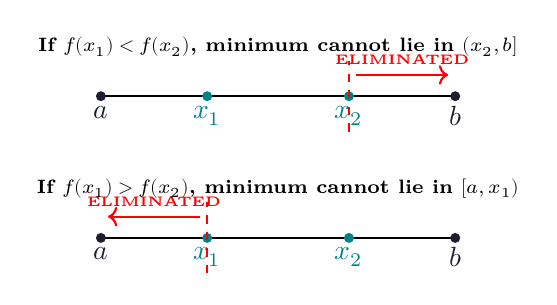
\begin{tikzpicture}[scale=0.9]
  % Case 1: f(x1) < f(x2)
  \draw[thick] (0,0) -- (5,0);
  \fill[mydark] (0,0) circle (2pt) node[below] {$a$};
  \fill[mydark] (5,0) circle (2pt) node[below] {$b$};
  \fill[myteal] (1.5,0) circle (2pt) node[below] {$x_1$};
  \fill[myteal] (3.5,0) circle (2pt) node[below] {$x_2$};
  \draw[dashed, red, thick] (3.5,-0.5) -- (3.5,0.5);
  \draw[red, ->, thick] (3.6, 0.3) -- (4.9, 0.3) node[midway, above, font=\tiny\bfseries] {ELIMINATED};
  \node[font=\scriptsize\bfseries] at (2.5, 0.7) {If $f(x_1) < f(x_2)$, minimum cannot lie in $(x_2, b]$};

  % Case 2: f(x1) > f(x2)
  \begin{scope}[yshift=-2.0cm]
    \draw[thick] (0,0) -- (5,0);
    \fill[mydark] (0,0) circle (2pt) node[below] {$a$};
    \fill[mydark] (5,0) circle (2pt) node[below] {$b$};
    \fill[myteal] (1.5,0) circle (2pt) node[below] {$x_1$};
    \fill[myteal] (3.5,0) circle (2pt) node[below] {$x_2$};
    \draw[dashed, red, thick] (1.5,-0.5) -- (1.5,0.5);
    \draw[red, ->, thick] (1.4, 0.3) -- (0.1, 0.3) node[midway, above, font=\tiny\bfseries] {ELIMINATED};
    \node[font=\scriptsize\bfseries] at (2.5, 0.7) {If $f(x_1) > f(x_2)$, minimum cannot lie in $[a, x_1)$};
  \end{scope}
\end{tikzpicture}
\end{tcolorbox}

\subsection{Interval Halving Method}
This method eliminates exactly half of the interval at each stage using three evaluations ($x_0$, $x_1$, and $x_2$).

\begin{tcolorbox}[formulabox, title={Interval Halving Algorithm}]
Let the current interval be $[a, b]$.
\begin{enumerate}[label=\textbf{\arabic*.}, leftmargin=*, itemsep=2pt, topsep=0pt]
  \item Calculate the midpoint: $x_0 = \frac{a+b}{2}$.
  \item Calculate quarter points:
    \begin{equation}
      x_1 = a + \frac{b-a}{4}, \quad x_2 = b - \frac{b-a}{4}
    \end{equation}
  \item Evaluate $f(x_1)$, $f(x_0)$, and $f(x_2)$.
  \item Compare function values to eliminate region:
    \begin{itemize}[label=\tiny$\bullet$, leftmargin=1.5em, itemsep=1.5pt]
      \item If $f(x_1) < f(x_0)$, the new interval is $[a, x_0]$.
      \item If $f(x_2) < f(x_0)$, the new interval is $[x_0, b]$.
      \item If $f(x_1) \ge f(x_0)$ and $f(x_2) \ge f(x_0)$, the new interval is $[x_1, x_2]$.
    \end{itemize}
  \item In all cases, the new interval width is exactly:
    \begin{equation}
      L_{new} = \frac{b-a}{2}
    \end{equation}
\end{enumerate}
\end{tcolorbox}

\subsection{Fibonacci Search Method}
Fibonacci search is the mathematically optimal region-elimination method. It uses the Fibonacci sequence $F_0 = 1$, $F_1 = 1$, $F_n = F_{n-1} + F_{n-2}$ to calculate placement ratios.

\begin{tcolorbox}[formulabox, title={Fibonacci Search Equations}]
For a pre-selected total number of function evaluations $n$:
\begin{enumerate}[label=\textbf{\arabic*.}, leftmargin=*, itemsep=3pt, topsep=0pt]
  \item The initial two test points $x_1$ and $x_2$ in $[a, b]$ are placed at:
    \begin{equation}
      x_1 = a + \frac{F_{n-2}}{F_n}(b - a)
    \end{equation}
    \begin{equation}
      x_2 = b - \frac{F_{n-2}}{F_n}(b - a) = a + \frac{F_{n-1}}{F_n}(b - a)
    \end{equation}
  \item After region elimination, the remaining sub-interval is evaluated. At the $k$-th step, the new test point is placed at:
    \begin{equation}
      x_k = \text{Remaining Limit} \pm \frac{F_{n-k-1}}{F_{n-k+1}}(\text{Current Interval Width})
    \end{equation}
  \item The final reduction ratio of the interval of uncertainty after $n$ iterations is:
    \begin{equation}
      \frac{L_n}{L_1} = \frac{1}{F_n}
    \end{equation}
\end{enumerate}
\end{tcolorbox}

% ===============================================================================
\section{Point Estimation Methods}
% ===============================================================================

Unlike region elimination, point estimation methods fit a smooth polynomial through known points to estimate the local minimum directly.

\subsection{Successive Quadratic Estimation (SQE)}
SQE fits a quadratic function $q(x) = A x^2 + B x + C$ through three test points $x_1 < x_2 < x_3$ with known function values $f_1, f_2, f_3$.

\begin{tcolorbox}[formulabox, title={SQE Minimum Point Formula}]
The minimum $x^*$ of the approximating quadratic polynomial is given by:
\begin{equation}
  x^* = \frac{1}{2} \frac{(x_2^2 - x_3^2)f_1 + (x_3^2 - x_1^2)f_2 + (x_1^2 - x_2^2)f_3}{(x_2 - x_3)f_1 + (x_3 - x_1)f_2 + (x_1 - x_2)f_3}
\end{equation}
\par\vspace{3pt}
Alternatively, we can express the calculation using coordinate differences:
\begin{equation}
  x^* = x_2 + \frac{1}{2} \frac{(x_2 - x_1)^2(f_2 - f_3) - (x_2 - x_3)^2(f_2 - f_1)}{(x_2 - x_1)(f_2 - f_3) - (x_2 - x_3)(f_2 - f_1)}
\end{equation}
If $x^*$ is close to $x_2$ within a tolerance limit, $x^*$ is taken as the optimum. Otherwise, the worst point among $\{x_1, x_2, x_3\}$ is replaced by $x^*$, and the calculation is repeated.
\end{tcolorbox}

\newpage

% ===============================================================================
% MANDATORY QUICK REVISION PAGE
% ===============================================================================
\begin{center}
  {\large\bfseries\color{myred} Quick Revision --- Module 2}\\[3pt]
  {\small\color{mydark} Single-Variable Optimization $|$ OE-EC704B}
\end{center}
\noindent{\color{myred}\rule{\linewidth}{1.2pt}}
\vspace{4pt}

\begin{tcolorbox}[formulabox, title={\textbf{Key Formulas \& Equations}}]
\renewcommand{\arraystretch}{1.45}
\begin{tabularx}{\linewidth}{B{5.0cm} X}
Necessary Condition & $f'(x^*) = 0$ \quad (stationary point requirement). \\[4pt]
Sufficient Condition & $f''(x^*) > 0 \implies \text{local min}$; $f''(x^*) < 0 \implies \text{local max}$. \\[4pt]
Interval Halving Width & $L_{new} = \frac{1}{2} L_{old}$ \quad (achieved with 3 evaluations). \\[4pt]
Fibonacci Point 1 & $x_1 = a + \frac{F_{n-2}}{F_n}(b-a)$. \\[4pt]
Fibonacci Reduction Ratio & $\frac{L_n}{L_1} = \frac{1}{F_n}$ \quad (where $F_n$ is the $n$-th Fibonacci number). \\[4pt]
SQE Minimum Point & $x^* = x_2 + \frac{1}{2} \frac{(x_2 - x_1)^2(f_2 - f_3) - (x_2 - x_3)^2(f_2 - f_1)}{(x_2 - x_1)(f_2 - f_3) - (x_2 - x_3)(f_2 - f_1)}$. \\
\end{tabularx}
\end{tcolorbox}

\begin{tcolorbox}[defbox, title={\textbf{One-Line Definitions}}]
\begin{itemize}[leftmargin=*, itemsep=2.5pt, topsep=0pt]
  \item \textbf{Stationary Point:} A point at which the first derivative of a differentiable function is zero.
  \item \textbf{Inflection Point:} A point on a curve at which the concavity changes, where $f''(x)=0$ and $f'''(x) \neq 0$.
  \item \textbf{Unimodal Function:} A function that has exactly one local extremum (minimum or maximum) in a given interval.
  \item \textbf{Bracketing Method:} A search algorithm designed to find an initial interval containing the optimum.
  \item \textbf{Region Elimination:} Systematically discarding a sub-interval of search space using unimodality comparisons.
  \item \textbf{Fibonacci Search:} An optimal region-elimination search algorithm utilizing Fibonacci ratios.
  \item \textbf{Successive Quadratic Estimation:} An interpolation algorithm that fits quadratic curves through test coordinates to locate the minimum.
\end{itemize}
\end{tcolorbox}

\begin{tcolorbox}[exambox, title={\textbf{Frequently Asked / Viva Questions}}]
\begin{enumerate}[topsep=0pt, label=\textbf{Q\arabic*.}, itemsep=5pt]
  \item \Q{State the necessary and sufficient conditions for a local minimum of a single-variable function.}
    Necessary condition: $f'(x^*) = 0$. Sufficient condition: $f''(x^*) > 0$.
  \item \Q{What happens if $f'(x^*) = f''(x^*) = 0$ at a candidate point?}
    The test is inconclusive. We must evaluate higher-order derivatives. If the first non-zero derivative is of odd order, it is an inflection point. If it is of even order and positive, it is a local minimum.
  \item \Q{Define a unimodal function and state why it is important for region-elimination methods.}
    A function is unimodal if it has only one optimum in a given range. Unimodality guarantees that comparing function values at two points ($f(x_1)$ and $f(x_2)$) yields a valid sub-region to eliminate.
  \item \Q{How does the Interval Halving method work?}
    It divides the interval into four equal parts using three points ($x_1 < x_0 < x_2$). Comparing their function values allows the elimination of half the interval ($L_{new} = 0.5 L_{old}$).
  \item \Q{Why is the Fibonacci search method considered optimal among region-elimination techniques?}
    For a pre-specified number of evaluations $n$, it achieves the maximum possible reduction in the interval of uncertainty ($1/F_n$) without requiring any derivative information.
  \item \Q{What is the relation between Fibonacci search and Golden Section search?}
    Golden Section search is the limiting case of Fibonacci search as the number of evaluations $n \to \infty$. It uses the constant Golden Ratio $\gamma \approx 0.618$ instead of discrete Fibonacci fractions.
  \item \Q{Write down the quadratic estimation formula for the minimum point $x^*$.}
    $x^* = \frac{1}{2} \frac{(x_2^2 - x_3^2)f_1 + (x_3^2 - x_1^2)f_2 + (x_1^2 - x_2^2)f_3}{(x_2 - x_3)f_1 + (x_3 - x_1)f_2 + (x_1 - x_2)f_3}$ for three ordered points $x_1 < x_2 < x_3$.
  \item \Q{Differentiate between bracketing methods and point estimation methods.}
    Bracketing methods find an interval containing the optimum (e.g., Exhaustive Search). Point estimation methods fit functional approximations (e.g., quadratic curves) to predict the exact coordinate of the optimum.
  \item \Q{Under what conditions does the successive quadratic estimation (SQE) method converge?}
    SQE converges rapidly if the objective function is smooth, continuous, and has a unimodal shape resembling a parabola in the neighborhood of the optimum.
  \item \Q{What is the significance of the Fibonacci numbers sequence in search algorithms?}
    The Fibonacci numbers satisfy the property $F_{n-2}/F_n \to 0.382$ and $F_{n-1}/F_n \to 0.618$, which balances the spacing of evaluation points so that previous calculations are reused in subsequent steps.
\end{enumerate}
\end{tcolorbox}

\end{document}
